\documentclass{article}
\usepackage{graphicx} % Required for inserting images

\title{Test 2}
\author{Klára Matějková}
\date{January 2025}

\begin{document}

\maketitle

\section{Damped Harmonic Oscillator}
A damped harmonic oscillator is a physical system that undergoes oscillatory motion while experiencing a damping force, which gradually reduces the amplitude of the oscillation over time. This type of system is commonly encountered in mechanical, electrical, and other physical contexts.

\subsection{Key Features of a Damped Harmonic Oscillator}
The system typically consists of a mass, a spring, and a damping element. The mass oscillates under the influence of a restoring force provided by the spring, which is proportional to displacement, as described by Hooke's law. The damping element introduces a resistive force proportional to the velocity, which opposes the motion and dissipates energy.

The motion of a damped harmonic oscillator is described by a second-order differential equation
\begin{equation}
    m\frac{d^2x}{dt^2}+b\frac{dx}{dt}+kx=0,
\end{equation}
where \emph{m} is the mass, \emph{b} is the damping coefficient, \emph{k} is the spring constant and \emph{x} is the displacement.

\subsection{Types of Damped Harmonic Oscillators}
The types of damped harmonic oscillators are categorized based on the \textbf{damping ratio $\zeta$}, which measures the relative strength of the damping compared to the system's natural oscillatory behavior. There are three primary types.
\begin{enumerate}
    \item Underdamped oscillators ($\zeta<1$)
    \item Overdamped oscillators ($\zeta>1$)
    \item Critically dumped iscillators ($\zeta=1$)
\end{enumerate}

\subsection{Solution to the Equation}
The general solution for displacement ${x(t)}$ depends on the damping ratio $(\zeta~=~\frac{b}{2\sqrt{mk}}$).
For \textbf{underdamped oscillations} it has a form
\begin{equation}
    x(t)=Ae^{-\zeta\omega_0t}cos(\omega_dt+\phi),
\end{equation}
where $\omega_0 = \sqrt{\frac{k}{m}}$ is the natural frequency, $\omega_d = \omega_0 \sqrt{1 - \zeta^2}$ is the damped frequency and $\phi$ is phase angle. The plot of position versus time for this solution is shown in Figure \ref{fig:Graph}.
\begin{figure}
    \centering
    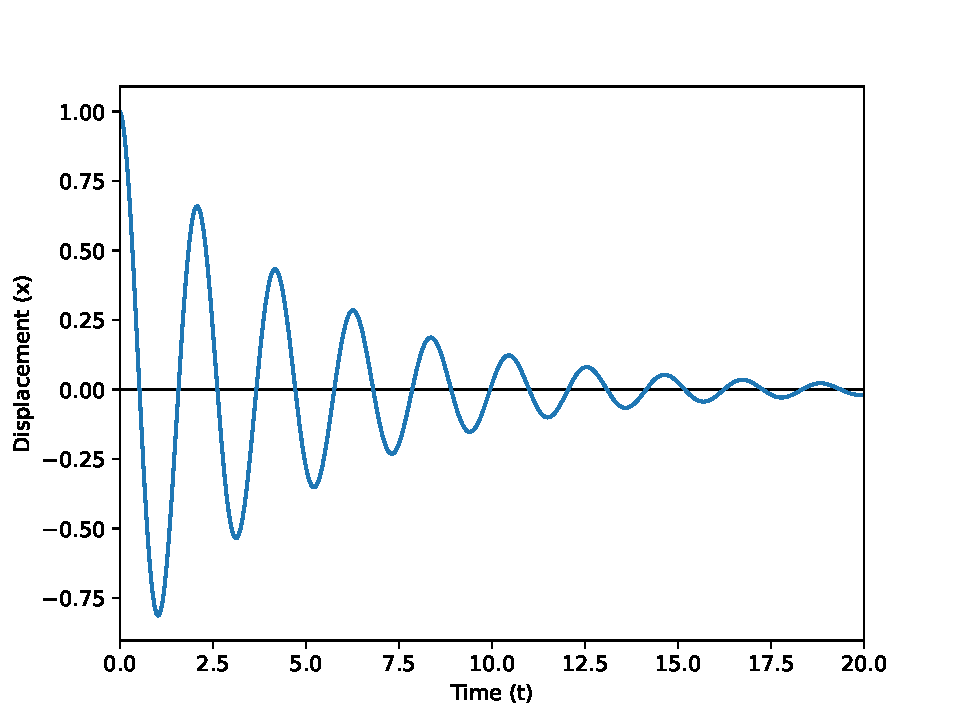
\includegraphics[width=0.7\linewidth]{dhs.pdf}
    \caption{Underdamped harmonic oscillator}
    \label{fig:Graph}
\end{figure}

In \textbf{critically damped systems}, the displacement takes the form 
\begin{equation}
    x(t)=(A+Bt)e^{-\omega_0t},
\end{equation}
while in \textbf{overdamped systems}, it is expressed as 
\begin{equation}
    x(t)=Ae^{r_1t}+Be^{r_2t},
\end{equation}
where $r_1$ and $r_2$ are the roots of the characteristic equation.

\subsection{Applications}
Damped harmonic oscillators have many practical applications. They are used in vehicle suspension systems, electrical RLC circuits, vibration isolation systems, and seismic dampers in buildings, among others. These applications rely on the system's ability to control oscillations and dissipate energy effectively.

\end{document}
